\documentclass[professionalfonts, aspectratio=169]{beamer}  
\usefonttheme{serif}                                        % Font theme: serif
\usepackage[utf8]{inputenc}                                 % Allows the use of different input encodings
\usepackage{graphicx}                                       % Enhanced support for graphics
\usepackage{amsmath}                                        % Enhances the typesetting of mathematics
\usepackage{amsfonts}                                       % Extra mathematical fonts
\usepackage{amssymb}                                        % Extra mathematical symbols
\usepackage{threeparttable}                 % For table notes
\usepackage{tikz}
\usetikzlibrary{shapes,arrows,positioning}
\usepackage{booktabs}                                       % Enhances the quality of tables
\usepackage{pgfplots}
\pgfplotsset{compat=1.17}
\usepackage{multirow}
% link settings
\usepackage{hyperref}                       % For hyperlinks
\usepackage[authoryear]{natbib}             % For bibliography

\usepackage{appendixnumberbeamer} % Numbering appendixes in beamer
\pdfstringdefDisableCommands{
  \def\translate{}
}
\usepackage{dcolumn}
\setbeamertemplate{navigation symbols}{} % Remove navigation symbols
\setbeamertemplate{footline}[frame number] % Add page number

% \setbeamercovered{transparent}  % Semi-transparent overlay

%---- Set the title page ----%
\title{Discussion on \\ ``Are Nutrient Policy Impacts on Recreation in Lake Erie \\ as Murky as the Water?''}
\institute{Stony Brook University}
\subtitle{by Farzaneh Sabbagh and Stephanie Brockmann}
\author{Zhu Liang}
\date{\today}

%---- Begin the document ----%
\begin{document}
\begin{frame}[plain]
  \titlepage
\end{frame}

\begin{frame}{Research Questions}
  \begin{figure}
    \centering
    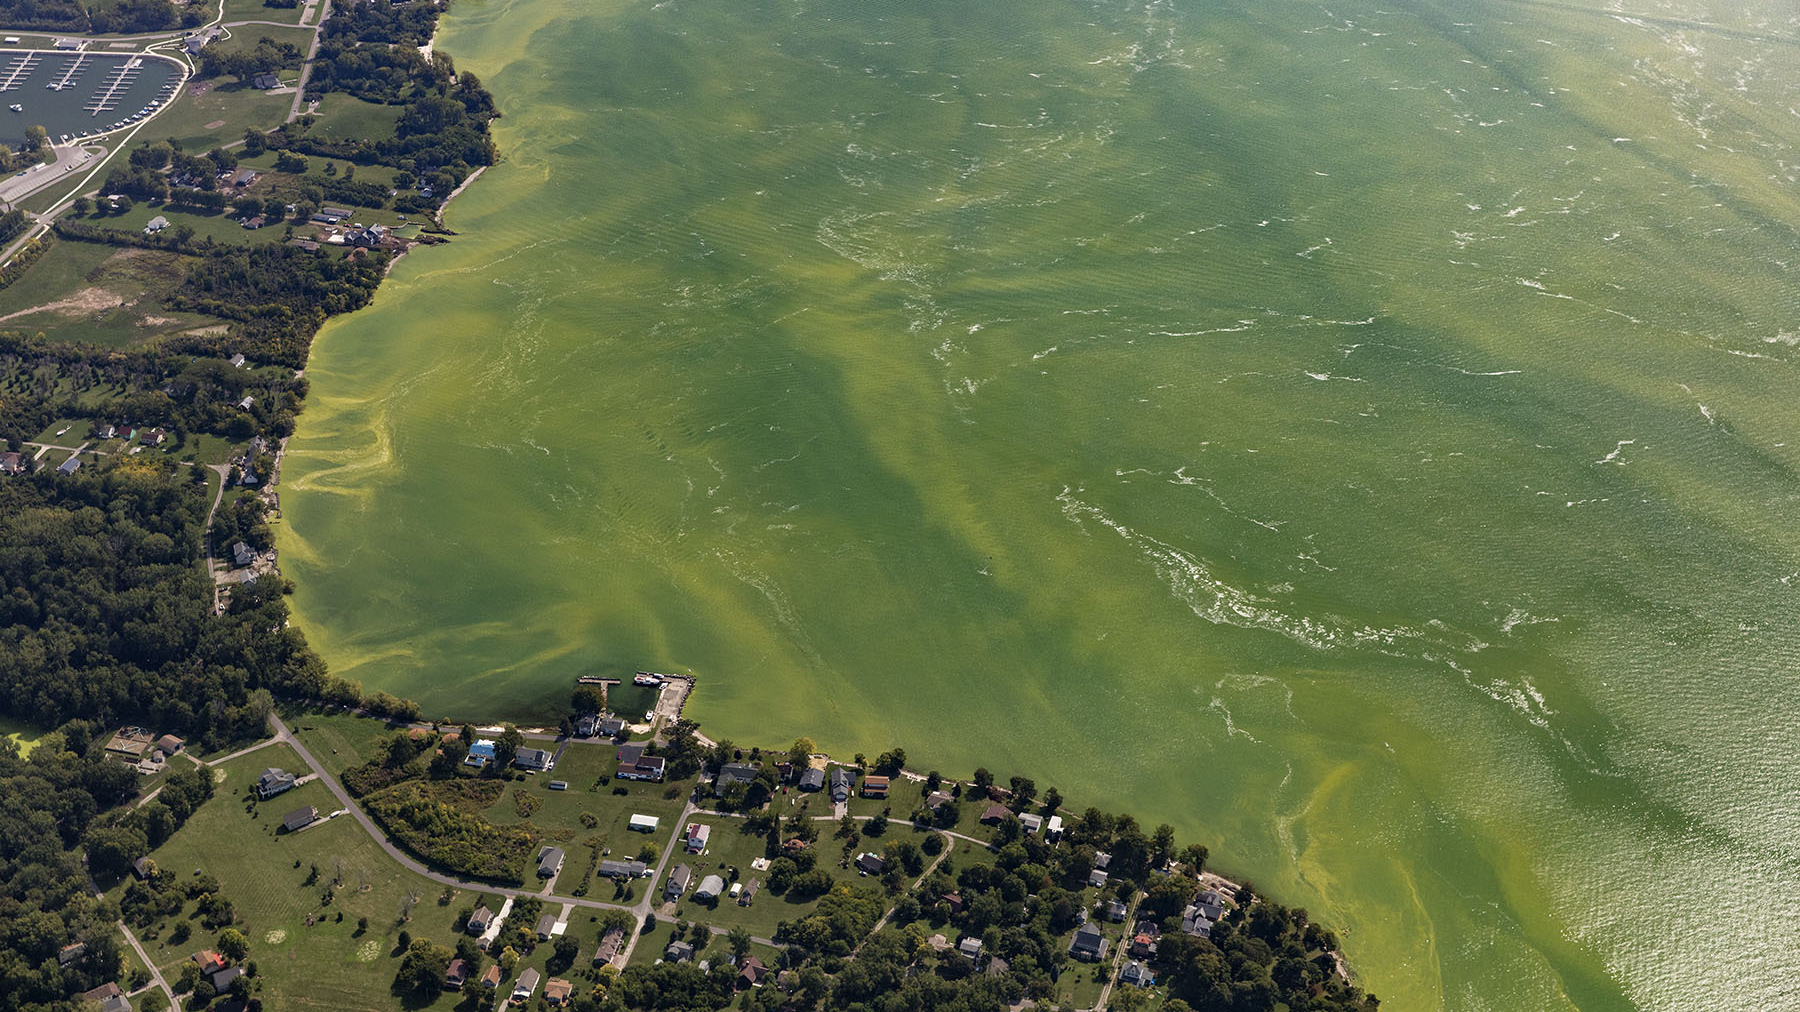
\includegraphics[width=0.5\linewidth]{habs.png}
    \caption{HABs By James Proffitt, Great Lakes Now, 2020}
  \end{figure}
  \begin{itemize}
      \item \textbf{Background:} Lake Erie has harmful algal blooms (HABs) from excess nutrients.
      \item \textbf{Problem:} HABs reduce water quality, impacting recreation and the economy.
      \item \textbf{Key Question:} How does a 40\% nutrient reduction policy affect recreation and economic outcomes?
  \end{itemize}
\end{frame}

\begin{frame}
  \frametitle{Contributions}
  \textbf{Methodology:}
  \begin{itemize}
    \item Integrated \textbf{economic} demand modeling (stated and revealed preferences) with \textbf{ecological} modeling outputs.
    \item Applied negative binomial regression to assess the sensitivity of recreational demand.
  \end{itemize}
\end{frame}

\begin{frame}
  \frametitle{Contributions}
  \textbf{Policy Implications:}
  \begin{itemize}
    \item \textbf{Spatial Heterogeneity:} Demonstrated that water quality impacts vary significantly based on geographic location and specific ecological dynamics.
    \item \textbf{Trade-offs:} Provided insights into the trade-offs between recreational benefits and economic costs (e.g., agricultural and fishing industries) resulting from nutrient policies.
  \end{itemize}
\end{frame}

\begin{frame}
  \frametitle{Potential Improvements}
  \begin{itemize}
    \item \textbf{Sample Limitation:} The study may be limited by its geographical and demographic scope.
    \item \textbf{Endogeneity Concerns:} Address potential endogeneity issues in estimating recreational demand as a function of ecological variables.
    \item \textbf{Pending Data:} Critical data (angler surveys and comprehensive ecological model results) are still pending.
  \end{itemize}
\end{frame}

\begin{frame}
  \frametitle{Conclusion}
  \begin{itemize}
    \item This study offers essential insights into the impacts of nutrient policies on recreational activities in Lake Erie.
    \item The findings highlight the necessity for adaptive management strategies to balance recreational benefits with potential economic costs.
  \end{itemize}
\end{frame}

\end{document}